% Provenance (never printed): see sources/outline_sources.md (Year 3:
% radial velocity, transits, imaging and microlensing; what has been
% found; atmospheres from transmission spectra).
% Brief: sources/book5/BRIEFS.md, ch. 28. Curves from figdata/bachelor-3/
% rv_transit.py (Keplerian radial-velocity curves, a limb-darkened transit
% light curve computed by numerical integration, point-lens microlensing)
% and exoplanet_archive.py (the NASA Exoplanet Archive's composite table of
% confirmed planets, fetched 2026-10-23, with the model mass--radius curves
% of Zeng et al.). Exercise and problem values in the Book 5 scratch
% calculator calc/ch28.py. Selene's Lamp and its planet are invented.
\chapter{Exoplanetas}\label{ch:b3:exoplanets}

No outono de 1994, dois astrônomos que mediam as velocidades de 142
estrelas constataram que uma delas, 51~Pegasi, se aproximava e se afastava
de nós com um período de cerca de quatro dias. A semiamplitude do movimento era
\qty{59}{m.s^{-1}}, quatro vezes o que o espectrógrafo deles podia detectar. O
companheiro que puxava a estrela tinha pelo menos metade da massa de
Júpiter, em uma órbita de \qty{0.05}{au}, oito vezes mais perto de sua estrela
do que Mercúrio está do Sol. Nenhuma teoria de formação planetária tinha lugar para
um corpo assim. A descoberta, anunciada em outubro de 1995, abriu um novo campo
da astronomia: três décadas depois, mais de seis mil planetas em torno de
outras estrelas estão confirmados, alguns deles foram observados diretamente, e a
atmosfera de alguns foi analisada. Este capítulo mostra como se encontram planetas
fracos demais para serem vistos, o que foi encontrado e como suas atmosferas
são lidas.
% ledger: nobel19:51peg, planet:Mercury.dist, data:b5-pscomp

\begin{recall}
O efeito Doppler, a velocidade radial, as binárias espectroscópicas, as leis de
Kepler, o problema de dois corpos e seu centro de massa, a lei de Planck e a
altura de escala de uma atmosfera isotérmica estão nos volumes de física.
Exoplaneta e zona habitável de uma estrela estão nos volumes escolares. O fluxo
e a luminosidade de uma fonte estão no volume do primeiro ano, no
capítulo sobre telescópios e fotometria; a temperatura de equilíbrio, no seu
capítulo de planetologia comparada. A formação planetária e a linha de neve
estão no volume do segundo ano. O \omterm{def:b3:planetary-atmospheres:jeans-escape}{escape de Jeans}, o \omterm{def:b3:planetary-atmospheres:hydrodynamic}{escape hidrodinâmico} e os
limites da zona habitável estão neste volume, no seu capítulo sobre
atmosferas planetárias.
\end{recall}

\section{O método da velocidade radial}\label{sec:b3:exoplanets:rv}

Um planeta não orbita sua estrela: os dois orbitam o centro de massa comum.
A estrela, muito mais pesada, descreve uma órbita pequena e própria, e sua luz
é deslocada por efeito Doppler, para um lado e para o outro, com o período do planeta.

\begin{definition}[Método da velocidade radial; massa mínima]\label{def:b3:exoplanets:rv}
O \emph{método da velocidade radial}\index{método da velocidade radial} detecta um
planeta pela variação periódica da velocidade radial de sua estrela,
medida a partir do deslocamento Doppler das linhas do espectro da estrela. Quando
a inclinação $i$ da órbita em relação ao plano do céu é desconhecida, mede-se
apenas o produto $m_p\sin i$ da massa do planeta pelo seno da inclinação, a
\emph{massa mínima}\index{massa mínima} do
planeta.
\end{definition}

\begin{theorem}[Semiamplitude da velocidade radial]\label{thm:b3:exoplanets:semi-amplitude}
Uma estrela de massa $M_\star$ e um planeta de massa $m_p$ em uma órbita circular de
período $P$ e inclinação $i$, dão à estrela uma velocidade radial
$v_r(t) = \gamma + K\cos\bigl(2\pi(t - t_0)/P\bigr)$, com $\gamma$ a
velocidade do centro de massa e a semiamplitude
\[
K = \left(\frac{2\pi G}{P}\right)^{1/3}
    \frac{m_p\sin i}{(M_\star + m_p)^{2/3}} .
\]
Em uma órbita de excentricidade $e$, a curva deixa de ser uma senoide,
$v_r = \gamma + K\bigl[\cos(\nu + \omega) + e\cos\omega\bigr]$, com $\nu$
a anomalia verdadeira e $\omega$ o argumento do periastro, e $K$ é
dividido por $\sqrt{1 - e^2}$.
\end{theorem}

\begin{proof}
Para a órbita circular: a separação $a$ dos dois corpos obedece
à terceira lei de Kepler, $a^3 = G(M_\star + m_p)P^2/4\pi^2$. A estrela está
à distância $a_\star = a\,m_p/(M_\star + m_p)$ do centro de massa e
percorre seu círculo com a velocidade $v_\star = 2\pi a_\star/P$. Daí
\[
v_\star = \frac{2\pi}{P}\,\frac{m_p}{M_\star + m_p}
          \left(\frac{G(M_\star + m_p)P^2}{4\pi^2}\right)^{1/3}
        = \left(\frac{2\pi G}{P}\right)^{1/3}\frac{m_p}{(M_\star + m_p)^{2/3}} .
\]
A linha de visada faz o ângulo $\pi/2 - i$ com o plano da
órbita, de modo que apenas $v_\star\sin i$ da velocidade da estrela está ao longo dela, e
essa componente gira com a estrela: $v_r - \gamma = v_\star\sin i\,
\cos\bigl(2\pi(t - t_0)/P\bigr)$. A forma excêntrica decorre da
elipse kepleriana e é aceita sem demonstração.
\end{proof}

Como o planeta é muito mais leve que sua estrela, $K$ fixa $m_p\sin i$
uma vez medido o período e conhecida a massa da estrela a partir de seu
espectro. Para 51~Pegasi~b, $K = \qty{59}{m.s^{-1}}$ e $P = \qty{4.23}{d}$
em torno de uma estrela de massa solar, dão $m_p\sin i = 0.47$ massas de Júpiter.
Júpiter move o Sol a \qty{12.5}{m.s^{-1}} ao longo de sua órbita de
\num{4331}~dias: um observador distante veria a velocidade do Sol oscilar cerca de
\qty{\pm 13}{m.s^{-1}} ao longo de doze anos. A Terra move o Sol a
\qty{9}{cm.s^{-1}}. O espectrógrafo que descobriu 51~Pegasi~b atingia
\qty{13}{m.s^{-1}}; seus sucessores chegam a cerca de \qty{1}{m.s^{-1}} (ou
seja, o ritmo de uma caminhada de \qty{3.5}{km/h}), e o mais recente é projetado para
\qty{10}{cm.s^{-1}}, suficiente para um planeta de massa terrestre na zona habitável
de uma estrela pouco massiva, onde a órbita do planeta é curta e a massa da estrela é baixa.
A própria estrela impõe um limite inferior: as pulsações e as manchas de sua superfície,
carregadas pela rotação, também deslocam suas linhas, e o sinal de um planeta
precisa ser distinguido delas.
% ledger: nobel19:51peg, nobel19:sun-jupiter, nobel19:migration, planet:Jupiter.mass, planet:Jupiter.Porb, planet:Jupiter.ecc, planet:Earth.mass, sun:mass, eso:espresso, const:G

\begin{omfigure}
\centering
\begin{tikzpicture}
\begin{axis}[width=0.86\linewidth, height=0.40\linewidth,
  xmin=0, xmax=2, ymin=-40, ymax=42,
  xlabel={fase orbital (em períodos)}, ylabel={$v_r - \gamma$ (\unit{m.s^{-1}})},
  tick label style={font=\scriptsize}, label style={font=\small},
  legend style={font=\scriptsize, at={(0.5,-0.30)}, anchor=north, legend columns=2, draw=none, cells={anchor=west}, /tikz/every even column/.append style={column sep=1em}}]
\addplot[thin, black!40, forget plot] coordinates {(0,0) (2,0)};
\addplot[thick, omDef] table[x=phase, y=v_circ] {figdata/out/bachelor-3-rv_transit-rv.dat};
\addlegendentry{órbita circular}
\addplot[thick, dashed, red!70!black] table[x=phase, y=v_ecc] {figdata/out/bachelor-3-rv_transit-rv.dat};
\addlegendentry{$e = 0.3$, $\omega = \ang{60}$}
\draw[<->, thick] (axis cs:1.0,0) -- (axis cs:1.0,30);
\node[font=\scriptsize, anchor=east] at (axis cs:0.99,12) {$K$};
\end{axis}
\end{tikzpicture}
\par\smallskip{\small A velocidade radial de uma estrela com um planeta, ao longo de
duas órbitas, para um planeta fictício com $K = \qty{30}{m.s^{-1}}$ e um
período de dez dias. Em uma órbita circular (linha contínua), a curva é uma senoide
de semiamplitude $K$. Em uma órbita excêntrica (tracejada), a estrela se move
mais rápido perto do periastro, e a curva torna-se assimétrica: seus extremos são
$K(1 \pm e\cos\omega)$ e a oscilação de pico a pico se mantém
$2K$.}\label{fig:b3:exoplanets:rv}
\end{omfigure}

\section{Trânsitos}\label{sec:b3:exoplanets:transits}

Se a órbita é vista quase de perfil, o planeta passa à frente de
sua estrela uma vez por órbita e oculta uma pequena parte de seu disco.

\begin{definition}[Método do trânsito; profundidade do trânsito; parâmetro de impacto]\label{def:b3:exoplanets:transit}
O \emph{método do trânsito}\index{método do trânsito} detecta um planeta pela
diminuição periódica do brilho de sua estrela quando o planeta cruza o disco estelar. A
\emph{profundidade do trânsito}\index{profundidade do trânsito} $\delta$ é a queda fracionária
do fluxo da estrela durante o trânsito. O \emph{parâmetro de
impacto}\index{parâmetro de impacto (trânsito)} $b = a\cos i/R_\star$ é a
menor distância entre os centros do planeta e da estrela, vista no céu,
em unidades do raio estelar $R_\star$, para uma órbita de raio
$a$ e inclinação $i$.
\end{definition}

\begin{proposition}[Profundidade do trânsito]\label{prop:b3:exoplanets:depth}
Um planeta escuro de raio $R_p$ inteiramente à frente de uma estrela de brilho uniforme
produz a profundidade $\delta = (R_p/R_\star)^2$.
\end{proposition}

\begin{proof}
O planeta oculta a área $\pi R_p^2$ de um disco de área $\pi R_\star^2$
igualmente brilhante em toda parte; o fluxo cai na mesma proporção.
\end{proof}

Júpiter cruzando o Sol o escureceria em \qty{1.06}{\percent}, a Terra
em \num{84} partes por milhão: o primeiro está ao alcance de um pequeno
telescópio, a segunda exige um telescópio espacial que meça milhares de
estrelas por anos. No entanto, um disco estelar não é uniforme.

\begin{definition}[Escurecimento do limbo]\label{def:b3:exoplanets:limb}
O \emph{escurecimento do limbo}\index{escurecimento do limbo} é a diminuição do
brilho superficial de uma estrela do centro de seu disco até a borda, o limbo.
Próximo ao limbo, a linha de visada entra na atmosfera da estrela obliquamente
e atinge profundidade óptica unitária em camadas mais altas e mais frias, que emitem
menos. Costuma-se escrevê-la como uma lei quadrática em $\mu = \cos\theta =
\sqrt{1 - r^2}$, com $r$ a distância do centro do disco em raios estelares:
$I(\mu)/I(1) = 1 - u_1(1 - \mu) - u_2(1 - \mu)^2$.
\end{definition}

Um planeta próximo ao centro de um disco com \omterm{def:b3:exoplanets:limb}{escurecimento do limbo} oculta luz
mais brilhante que a média e aprofunda o trânsito; próximo ao limbo, oculta menos. O
fundo da curva de luz torna-se arredondado, e suas bordas se suavizam. A duração
de um trânsito carrega a geometria.

\begin{theorem}[Duração do trânsito]\label{thm:b3:exoplanets:duration}
Para uma órbita circular de período $P$, raio $a$ e inclinação $i$, com
$p = R_p/R_\star$ e \omterm{def:b3:exoplanets:transit}{parâmetro de impacto} $b$, o tempo desde o primeiro
contato até o último é
\[
T_{14} = \frac{P}{\pi}\arcsin\!\left(\frac{R_\star}{a}\,
          \frac{\sqrt{(1 + p)^2 - b^2}}{\sin i}\right),
\]
e o tempo entre o segundo e o terceiro contatos, quando o planeta está
inteiramente dentro do disco, $T_{23}$, é dado pela mesma fórmula com
$1 - p$ no lugar de $1 + p$.
\end{theorem}

\begin{proof}
Seja $\varphi = 2\pi t/P$ a fase orbital contada a partir do meio do trânsito.
Projetado no céu, com $x$ ao longo da trajetória do planeta e $y$ transversalmente a ela,
o centro do planeta está em $x = a\sin\varphi$ e $y = a\cos i\cos\varphi$
em relação ao centro da estrela. Em raios estelares, o quadrado da separação é
\[
z^2 = \left(\frac{a}{R_\star}\right)^2(\sin^2\varphi + \cos^2 i\cos^2\varphi)
    = \left(\frac{a}{R_\star}\right)^2\sin^2 i\,\sin^2\varphi + b^2 .
\]
Os discos se tocam por fora quando $z = 1 + p$, em
$\sin\varphi = \sqrt{(1 + p)^2 - b^2}\,R_\star/(a\sin i)$, simétrico
em relação ao meio do trânsito. O trânsito dura a fase $2\varphi$, isto é, o
tempo $2\varphi P/2\pi = P\varphi/\pi$. Com $z = 1 - p$, os discos se tocam
por dentro.
\end{proof}

Para uma órbita larga, o arco-seno é o seu próprio argumento: $T_{14} \approx (P/\pi)
(R_\star/a)\sqrt{(1 + p)^2 - b^2}$. Um trânsito central dura mais; um
rasante, com $b$ próximo de $1 + p$, é curto e tem forma de V. Medindo
$T_{14}$ e $T_{23}$ em uma curva de luz, obtêm-se $b$ e $a/R_\star$, logo
a inclinação: o trânsito elimina o $\sin i$ que a velocidade radial
deixa desconhecido.

\begin{omfigure}
\centering
\begin{tikzpicture}[scale=0.92]
\shade[inner color=yellow!25, outer color=orange!70] (0,0) circle (2);
\draw[orange!70!black] (0,0) circle (2);
\draw[dashed, black!60] (-3.2,-0.6) -- (3.2,-0.6);
\draw[->, black!60] (2.5,-0.6) -- (3.2,-0.6) node[right, font=\scriptsize] {trajetória};
\foreach \x in {-2.117, -1.697, 1.697, 2.117} {\fill[black] (\x,-0.6) circle (0.2);}
\node[font=\scriptsize] at (-2.117,-1.0) {1};
\node[font=\scriptsize] at (-1.697,-0.2) {2};
\node[font=\scriptsize] at (1.697,-0.2) {3};
\node[font=\scriptsize] at (2.117,-1.0) {4};
\fill[black] (0,0) circle (0.03);
\draw[<->, thick, omDef] (0,0) -- (0,-0.6) node[midway, left, font=\scriptsize] {$bR_\star$};
\draw[->] (0,0) -- (1.414,1.414) node[midway, above left, font=\scriptsize] {$R_\star$};
\end{tikzpicture}\hfill
\begin{tikzpicture}
\begin{axis}[width=0.52\linewidth, height=0.42\linewidth,
  xmin=-4, xmax=4, ymin=0.9855, ymax=1.0025,
  xlabel={tempo a partir do meio do trânsito (h)}, ylabel={fluxo relativo},
  yticklabel style={/pgf/number format/fixed, /pgf/number format/precision=3},
  tick label style={font=\scriptsize}, label style={font=\small},
  legend style={font=\scriptsize, at={(0.5,-0.30)}, anchor=north, legend columns=1, draw=none, cells={anchor=west}, /tikz/every even column/.append style={column sep=1em}}]
\addplot[thick, omDef] table[x=t_h, y=flux_ld] {figdata/out/bachelor-3-rv_transit-transit.dat};
\addlegendentry{estrela com escurecimento do limbo}
\addplot[thick, dashed, black!60] table[x=t_h, y=flux_uni] {figdata/out/bachelor-3-rv_transit-transit.dat};
\addlegendentry{estrela uniforme}
\draw[densely dotted, black!50] (axis cs:-2.698,0.9855) -- (axis cs:-2.698,1.0025);
\node[font=\scriptsize, anchor=south] at (axis cs:-2.698,1.0005) {1};
\draw[densely dotted, black!50] (axis cs:-2.162,0.9855) -- (axis cs:-2.162,1.0025);
\node[font=\scriptsize, anchor=south] at (axis cs:-2.162,1.0005) {2};
\draw[densely dotted, black!50] (axis cs:2.162,0.9855) -- (axis cs:2.162,1.0025);
\node[font=\scriptsize, anchor=south] at (axis cs:2.162,1.0005) {3};
\draw[densely dotted, black!50] (axis cs:2.698,0.9855) -- (axis cs:2.698,1.0025);
\node[font=\scriptsize, anchor=south] at (axis cs:2.698,1.0005) {4};
\end{axis}
\end{tikzpicture}
\par\smallskip{\small À esquerda: um planeta com $p = R_p/R_\star = 0.1$ cruza
o disco de sua estrela no \omterm{def:b3:exoplanets:transit}{parâmetro de impacto} $b = 0.3$, nos quatro
contatos 1 a 4; o disco é mais escuro em direção ao limbo. À direita: a curva
de luz para $a/R_\star = 15$ e período de dez dias, calculada para uma estrela
com os coeficientes quadráticos de \omterm{def:b3:exoplanets:limb}{escurecimento do limbo} $u_1 = 0.40$, $u_2 = 0.25$
(linha contínua) e para uma estrela uniforme (tracejada, profundidade exatamente $p^2 = 1\,\%$).
Entre os contatos 2 e 3 a curva com \omterm{def:b3:exoplanets:limb}{escurecimento do limbo} é arredondada e
mais profunda que $p^2$ próximo ao meio do trânsito.}\label{fig:b3:exoplanets:transit}
\end{omfigure}

\begin{proposition}[Probabilidade de trânsito]\label{prop:b3:exoplanets:probability}
Um planeta em órbita circular de raio $a$, orientada ao acaso, transita
sua estrela (com $b < 1$) com probabilidade $R_\star/a$.
\end{proposition}

\begin{proof}
Para órbitas orientadas ao acaso, $\cos i$ tem distribuição uniforme entre
0 e 1. O planeta transita quando $b = (a/R_\star)\cos i < 1$, ou seja
quando $\cos i < R_\star/a$, o que ocorre com probabilidade $R_\star/a$.
\end{proof}

Um observador distante veria a Terra transitar diante do Sol com probabilidade
de \qty{0.47}{\percent}, Júpiter com \qty{0.09}{\percent}. Um levantamento por
trânsito enxerga apenas uma pequena fração dos planetas em torno das estrelas que
observa, e sobretudo os mais próximos da estrela.

Cada método, isoladamente, deixa algo de fora. A velocidade radial fornece
$m_p\sin i$; o trânsito fornece $R_p/R_\star$ e $i$. Juntos, eles fornecem
a massa verdadeira e o raio, e daí a densidade média
$\bar\rho = 3m_p/4\pi R_p^3$, a primeira pista sobre a composição de um planeta.
Os primeiros trânsitos, relatados no início de 2000, foram os de um planeta
já conhecido pela velocidade de sua estrela, HD~209458~b. Seus dois trânsitos
mostraram o \omterm{def:b3:exoplanets:limb}{escurecimento do limbo} da estrela e deram um raio de 1.27 raios de Júpiter, com inclinação de
\ang{87.1}. Com a massa e o raio do arquivo, sua densidade média é
\qty{0.34}{g.cm^{-3}}, um terço da densidade da água: um gigante gasoso inflado pelo
calor da estrela.
% ledger: planet:Jupiter.diameter, planet:Earth.diameter, sun:R, const:au, planet:Jupiter.dist, charbonneau00:hd209458, nobel19:transits, data:b5-pscomp

Um planeta que transita funciona como um relógio. Se um segundo planeta o puxa, seus
trânsitos chegam adiantados ou atrasados, em um padrão que se repete com a
interação gravitacional.

\begin{definition}[Variação do tempo de trânsito]\label{def:b3:exoplanets:ttv}
Uma \emph{variação do tempo de trânsito}\index{variação do tempo de trânsito} é o
desvio dos instantes dos trânsitos de um planeta em relação a uma sequência estritamente periódica,
sequência causado pela atração gravitacional de outro corpo do
sistema; ela pode revelar, e pesar, planetas que não transitam por
si mesmos.
\end{definition}

Uma queda na curva de luz nem sempre é um planeta. Um par de estrelas eclipsantes
que tangencia, ou um par eclipsante tênue atrás do alvo cuja
luz é diluída pela do alvo, pode imitar um trânsito. Um candidato torna-se
um planeta quando sua massa é medida, pela velocidade radial ou pelas variações
de tempo, ou quando todas as outras explicações foram descartadas.

\section{Imageamento e microlente}\label{sec:b3:exoplanets:imaging}

\begin{definition}[Imageamento direto; coronógrafo]\label{def:b3:exoplanets:imaging}
O \emph{imageamento direto}\index{imageamento direto} detecta um planeta por sua própria
luz, refletida ou emitida, separada no céu da luz de sua
estrela. Um \emph{coronógrafo}\index{coronógrafo} é um instrumento que bloqueia
a luz da estrela no foco do telescópio, por meio de uma máscara ou pela
interferência da luz, de modo que fontes tênues próximas da estrela possam ser
vistas.
\end{definition}

A dificuldade é dupla. Uma órbita de \qty{1}{au} vista a partir de \qty{10}{pc}
ocupa apenas \ang{;;0.1}, e o planeta é muitas ordens de grandeza mais tênue
que sua estrela. Planetas gigantes jovens são os alvos mais fáceis: ainda quentes da
formação, brilham no infravermelho, onde o contraste com a estrela é
menor. Em 2008, imagens obtidas em dois grandes telescópios mostraram três
planetas em torno da estrela HR~8799, com separações projetadas de 24, 38 e
\qty{68}{au}, movendo-se no sentido anti-horário de um ano para o seguinte; sua
baixa luminosidade e a idade do sistema lhes atribuem de 5 a 13
massas de Júpiter. O planeta da fotografia abaixo dista \ang{;;0.82} de sua
estrela; os \omterm{def:b3:exoplanets:imaging}{coronógrafos} do telescópio espacial atingem um contraste de
\num{1e-5} a \ang{;;1} em \qty{4.4}{\micro m}.
% ledger: iau:parsec, const:au, marois08:hr8799, carter23:hip65426

\begin{omfigure}
\centering
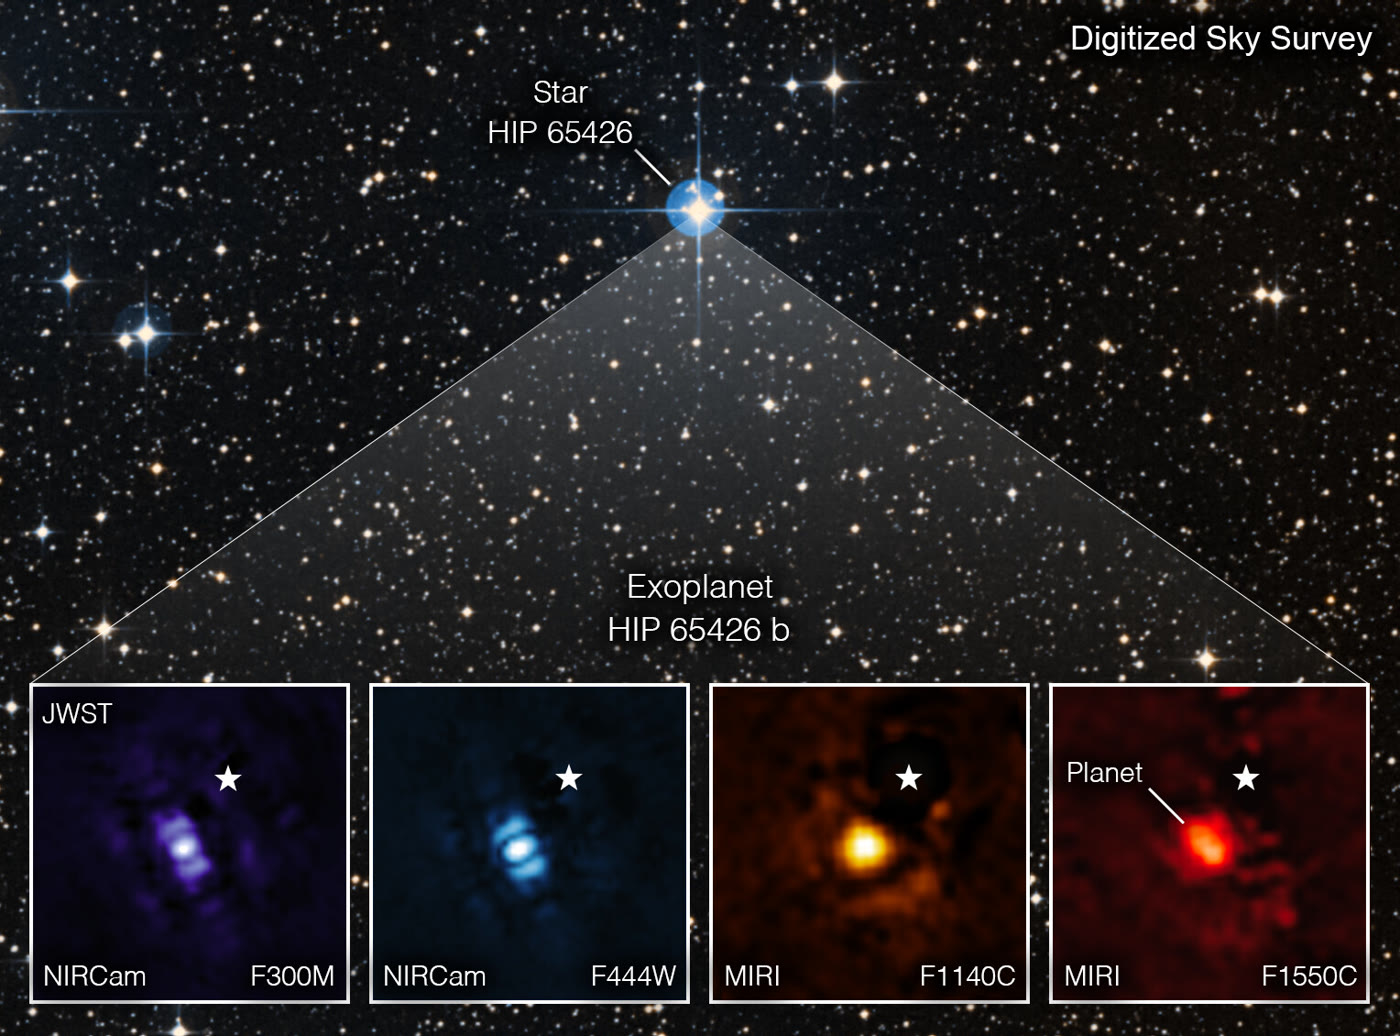
\includegraphics[width=0.86\linewidth]{images/book5/b3-hip65426b.jpg}
\par\smallskip{\small O primeiro exoplaneta imageado pelo James Webb Space
Telescope, HIP~65426~b, em quatro filtros infravermelhos (embaixo; em cima, o
campo da estrela em um levantamento do céu feito do solo); a luz da
estrela, na posição do símbolo da estrela, é bloqueada pelos
\omterm{def:b3:exoplanets:imaging}{coronógrafos}. O planeta é um gigante gasoso jovem, de cerca de 6 a 8
massas de Júpiter, com cerca de 15 a 20 milhões de anos, e situado cerca de cem vezes
mais longe de sua estrela do que a Terra do Sol. Imagem NASA/ESA/CSA,
A~Carter (UCSC), a equipe ERS~1386, e A.~Pagan (STScI), CC
BY~4.0.}\label{fig:b3:exoplanets:hip65426}
\end{omfigure}
% ledger: photo:b3-hip65426b

Um quarto método usa a gravidade como lente. Quando uma estrela passa quase exatamente
na frente de outra mais distante, sua gravidade curva a luz da
estrela de fundo e a torna mais brilhante por algumas semanas; um planeta da estrela que
atua como lente acrescenta um breve pico de brilho.

\begin{definition}[Microlente gravitacional; raio de Einstein]\label{def:b3:exoplanets:microlensing}
A \emph{microlente gravitacional}\index{microlente gravitacional} é o
aumento temporário do brilho de uma estrela de fundo quando uma estrela em primeiro plano, a
lente, passa perto da linha de visada; as imagens que ela forma estão próximas demais
para serem resolvidas. O \emph{raio de Einstein}\index{raio de Einstein}
é o raio angular $\theta_\mathrm E$ do anel no qual uma lente pontual
de massa $M$ à distância $D_L$ faria uma fonte à
distância $D_S$ exatamente atrás dela:
\[
\theta_\mathrm E = \sqrt{\frac{4GM}{c^2}\,\frac{D_S - D_L}{D_L D_S}} .
\]
\end{definition}

\begin{proposition}[Amplificação de lente pontual]\label{prop:b3:exoplanets:magnification}
Uma fonte à distância angular $u\,\theta_\mathrm E$ de uma lente pontual
tem seu brilho multiplicado pelo fator
\[
A(u) = \frac{u^2 + 2}{u\sqrt{u^2 + 4}} .
\]
\end{proposition}

\admitted

Ambos os resultados decorrem do desvio da luz por uma massa na
relatividade geral. Para uma lente de meia massa solar a meio caminho de uma fonte
situada a \qty{8}{kpc} de distância, $\theta_\mathrm E = \qty{0.71}{mas}$, e o anel de
Einstein, à distância da lente, tem raio de \qty{2.9}{au}. Em
$u = 1$ a fonte tem seu brilho multiplicado por 1.34, e, em $u = 0.1$, por dez. Um
planeta próximo ao anel de Einstein de sua estrela acrescenta um breve desvio à
curva de luz. Assim, a microlente encontra planetas a poucas unidades astronômicas
de suas estrelas, planetas frios que trânsitos e velocidades radiais não detectam,
mas cada evento acontece uma única vez e nunca se repete. Em um evento de 2003,
publicado no ano seguinte, um desvio com duração de cerca de sete dias foi
explicado somente por uma companheira de $\num{0.0039}$ vezes a massa da
lente: um planeta de cerca de 1.5 massas de Júpiter, a cerca de \qty{3}{au} de sua
estrela.
% ledger: const:G, const:c, sun:mass, iau:parsec, const:au, bond04:ogle235

\begin{omfigure}
\centering
\begin{tikzpicture}[scale=0.95]
\fill (0,0) circle (0.06) node[below=2pt, font=\scriptsize] {fonte};
\fill[omDef] (3.2,0) circle (0.09); \node[font=\scriptsize, omDef] at (3.2,-1.15) {lente};
\draw[omDef] (3.2,0) ellipse (0.12 and 0.9);
\fill (6.4,0) circle (0.06) node[below=2pt, font=\scriptsize] {observador};
\draw[thick, orange!80!black] (0,0) -- (3.2,0.9) -- (6.4,0);
\draw[thick, orange!80!black] (0,0) -- (3.2,-0.9) -- (6.4,0);
\draw[densely dashed, black!50] (6.4,0) -- (0,1.8) node[left, font=\scriptsize] {imagem};
\draw[densely dotted, black!50] (0,0) -- (6.4,0);
\draw[<->] (3.55,0) -- (3.55,0.9) node[midway, right, font=\scriptsize] {$R_\mathrm E$};
\draw[<->, black!60] (0,-1.5) -- (3.2,-1.5) node[midway, below, font=\scriptsize] {$D_S - D_L$};
\draw[<->, black!60] (3.2,-1.5) -- (6.4,-1.5) node[midway, below, font=\scriptsize] {$D_L$};
\end{tikzpicture}\hfill
\begin{tikzpicture}
\begin{axis}[width=0.48\linewidth, height=0.42\linewidth,
  xmin=-3, xmax=3, ymin=0.8, ymax=12, ymode=log,
  ytick={1,2,5,10}, yticklabels={1,2,5,10},
  xlabel={tempo ($t_\mathrm E$)}, ylabel={magnificação $A$},
  tick label style={font=\scriptsize}, label style={font=\small},
  legend style={font=\scriptsize, at={(0.5,-0.30)}, anchor=north, legend columns=3, draw=none, cells={anchor=west}, /tikz/every even column/.append style={column sep=1em}}]
\addplot[thick, omDef] table[x=t_tE, y=A01] {figdata/out/bachelor-3-rv_transit-lens.dat};
\addlegendentry{$u_0 = 0.1$}
\addplot[thick, dashed, red!70!black] table[x=t_tE, y=A03] {figdata/out/bachelor-3-rv_transit-lens.dat};
\addlegendentry{$0.3$}
\addplot[thick, dotted, black] table[x=t_tE, y=A10] {figdata/out/bachelor-3-rv_transit-lens.dat};
\addlegendentry{$1$}
\end{axis}
\end{tikzpicture}
\par\smallskip{\small Esquerda: a geometria de uma lente gravitacional, fora de
escala; os raios da fonte passam pela lente em torno do \omterm{def:b3:exoplanets:microlensing}{raio de Einstein}
$R_\mathrm E = \theta_\mathrm E D_L$ e chegam ao observador, que vê a
fonte deslocada para a imagem. Direita: a amplificação de uma fonte pontual
por uma lente pontual em função do tempo, em unidades do tempo $t_\mathrm E$ que a lente
leva para se deslocar de um \omterm{def:b3:exoplanets:microlensing}{raio de Einstein}, para três distâncias de maior
aproximação $u_0$ (em \omterm{def:b3:exoplanets:microlensing}{raios de Einstein}).}\label{fig:b3:exoplanets:microlensing}
\end{omfigure}

Cada método tem seu próprio viés, e o catálogo de planetas conhecidos
reflete-os. As velocidades radiais favorecem planetas massivos próximos de suas
estrelas; os trânsitos favorecem planetas grandes próximos de suas estrelas, e exigem que a
órbita esteja de perfil; a microlente encontra planetas de poucas unidades astronômicas;
o imageamento encontra gigantes jovens situados a dezenas ou centenas de unidades astronômicas.
A figura abaixo mostra o resultado: cada método ocupa sua própria região, e
os planetas do Sistema Solar caem sobretudo nas lacunas entre elas.

\begin{dated}{2026}
Em 23 de outubro de 2026, o NASA Exoplanet Archive listava 6451 planetas
confirmados. Por método de descoberta: 4785 por trânsito, 1204 por
velocidade radial, 292 por microlente, 98 por imageamento, 29 por \omterm{def:b3:exoplanets:ttv}{variações do
tempo de trânsito} e os demais por métodos mais raros, entre eles os primeiros de
todos, encontrados em 1992 em torno de um pulsar pela cronometragem de seus pulsos. As
primeiras descobertas por velocidade radial datam de 1995, por trânsito de 2002, por
microlente e imageamento de 2004.
\end{dated}
% ledger: data:b5-pscomp

\begin{omfigure}
\centering
\begin{tikzpicture}
\begin{axis}[width=0.86\linewidth, height=0.56\linewidth,
  xmode=log, ymode=log, xmin=0.004, xmax=2000, ymin=0.02, ymax=1e5,
  legend image post style={scale=2.2},
  xlabel={semieixo maior (au)}, ylabel={massa ou massa mínima ($M_\oplus$)},
  tick label style={font=\scriptsize}, label style={font=\small},
  legend style={font=\scriptsize, at={(0.5,-0.20)}, anchor=north, legend columns=4, draw=none, cells={anchor=west}, /tikz/every even column/.append style={column sep=1em}}]
\addplot[only marks, mark=*, mark size=0.6pt, omDef, opacity=0.6] table[x=a_au, y=mass] {figdata/out/bachelor-3-exoplanet_archive-ma-tr.dat};
\addlegendentry{trânsito}
\addplot[only marks, mark=*, mark size=0.6pt, red!70!black, opacity=0.6] table[x=a_au, y=mass] {figdata/out/bachelor-3-exoplanet_archive-ma-rv.dat};
\addlegendentry{velocidade radial}
\addplot[only marks, mark=triangle*, mark size=1.2pt, green!45!black] table[x=a_au, y=mass] {figdata/out/bachelor-3-exoplanet_archive-ma-ml.dat};
\addlegendentry{microlente}
\addplot[only marks, mark=diamond*, mark size=1.5pt, orange!85!black] table[x=a_au, y=mass] {figdata/out/bachelor-3-exoplanet_archive-ma-im.dat};
\addlegendentry{imageamento}
\addplot[only marks, mark=square*, mark size=1.6pt, black, forget plot] table[x=a_au, y=mass] {figdata/out/bachelor-3-exoplanet_archive-solar.dat};
\node[font=\scriptsize, anchor=west, fill=white, inner sep=1pt] at (axis cs:1.15,1.0) {Terra};
\node[font=\scriptsize, anchor=east, fill=white, inner sep=1pt] at (axis cs:0.63,0.82) {Vênus};
\node[font=\scriptsize, anchor=east, fill=white, inner sep=1pt] at (axis cs:0.34,0.055) {Mercúrio};
\node[font=\scriptsize, anchor=west, fill=white, inner sep=1pt] at (axis cs:1.75,0.107) {Marte};
\node[font=\scriptsize, anchor=west, fill=white, inner sep=1pt] at (axis cs:6.0,318) {Júpiter};
\node[font=\scriptsize, anchor=west, fill=white, inner sep=1pt] at (axis cs:11,95) {Saturno};
\node[font=\scriptsize, anchor=north, fill=white, inner sep=1pt] at (axis cs:25,11) {Urano, Netuno};
\end{axis}
\end{tikzpicture}
\par\smallskip{\small Planetas confirmados com massa medida (ou \omterm{def:b3:exoplanets:rv}{massa mínima})
e semieixo maior, por método de descoberta (NASA Exoplanet
Archive, 23 de outubro de 2026: 1691 por trânsito, 1151 por velocidade radial, 286
por microlente, 94 por imageamento), com os planetas do Sistema Solar (quadrados
pretos). Massas previstas a partir de uma \omterm{def:b3:exoplanets:mass-radius}{relação massa--raio} ficam de fora. Esta pesquisa
fez uso do NASA Exoplanet Archive, operado pelo
California Institute of Technology, sob contrato com a National
Aeronautics and Space Administration, no âmbito do Exoplanet Exploration
Program.}\label{fig:b3:exoplanets:methods}
\end{omfigure}
% ledger: data:b5-pscomp, planet:Mercury.mass, planet:Venus.mass, planet:Earth.mass, planet:Mars.mass, planet:Jupiter.mass, planet:Saturn.mass, planet:Uranus.mass, planet:Neptune.mass, planet:Mercury.dist, planet:Venus.dist, planet:Earth.dist, planet:Mars.dist, planet:Jupiter.dist, planet:Saturn.dist, planet:Uranus.dist, planet:Neptune.dist

\section{O que foi encontrado}\label{sec:b3:exoplanets:found}

A primeira surpresa foram os \omterm{def:b3:exoplanets:classes}{Júpiteres quentes}, planetas gigantes em órbitas de
poucos dias. 51~Pegasi~b não pode ter se formado tão perto de sua estrela; ele deve
ter se formado mais para fora, talvez a algumas unidades astronômicas, além da
linha de neve de seu disco, e migrou para dentro por meio de sua interação com
o disco, como a teoria havia previsto.
% ledger: nobel19:migration

\begin{definition}[Júpiter quente; superterra; subnetuno]\label{def:b3:exoplanets:classes}
Um \emph{Júpiter quente}\index{Júpiter quente} é um planeta gigante em uma órbita próxima,
geralmente tomado como tendo \omterm{def:b3:exoplanets:rv}{massa mínima} acima de 0.1 massa de Júpiter e período
menor que dez dias. Uma \emph{superterra}\index{superterra} é um planeta
maior que a Terra, mas menor que o \omterm{def:b3:exoplanets:radius-valley}{vale de raios}, ou seja, de até
cerca de 1.5 a 2 raios terrestres, e portanto provavelmente rochoso. Um \emph{subnetuno}\index{subnetuno}
é um planeta acima do \omterm{def:b3:exoplanets:radius-valley}{vale de raios}, mas menor que Netuno, com cerca de 2 a
4 raios terrestres, cujo raio exige um envelope de gases leves ou
voláteis.
\end{definition}
% ledger: wright12:hj, fulton17:gap, planet:Neptune.diameter, planet:Earth.diameter

\begin{definition}[Taxa de ocorrência]\label{def:b3:exoplanets:occurrence}
A \emph{taxa de ocorrência}\index{taxa de ocorrência} de uma classe de planetas é
o número médio de tais planetas por estrela, ou a fração de estrelas que
abrigam um, em uma dada faixa de tamanho (ou massa) e período, após a
correção das contagens de um levantamento pelos planetas que ele não pôde detectar:
aqueles cujas órbitas não estão alinhadas para um trânsito, e aqueles pequenos demais ou
distantes demais para serem vistos.
\end{definition}

Os \omterm{def:b3:exoplanets:classes}{Júpiteres quentes}, em destaque no catálogo por serem os mais fáceis de
encontrar, são raros: um levantamento por velocidade radial de estrelas próximas e semelhantes ao Sol encontrou
deles em torno de \qty[separate-uncertainty=true]{1.2 \pm 0.38}{\percent} das estrelas. Planetas pequenos são
comuns. Ao pesquisar as curvas de luz de \num{42000} estrelas observadas pelo
telescópio espacial Kepler, um estudo encontrou 603 planetas, dez deles de tamanho terrestre (de 1 a 2
raios terrestres) e recebendo entre uma e quatro vezes a luz que a Terra
recebe do Sol; corrigido pela probabilidade de trânsito e pelos planetas que a
busca não detectaria, \qty[separate-uncertainty=true]{11 \pm 4}{\percent} das estrelas semelhantes ao Sol abrigam
um planeta desse tipo.
% ledger: wright12:hj, petigura13:eta

Os tamanhos dos planetas pequenos não se distribuem de modo uniforme. Entre os planetas de órbita próxima
medidos com precisão, os de 1.5 a 2.0 raios terrestres são pelo menos duas vezes
mais raros do que os imediatamente menores ou imediatamente maiores.

\begin{definition}[Vale de raios]\label{def:b3:exoplanets:radius-valley}
O \emph{vale de raios}\index{vale de raios} é o déficit de planetas
com raios entre cerca de 1.5 e 2.0 raios terrestres entre os planetas com
períodos menores que cerca de cem dias; ele separa as \omterm{def:b3:exoplanets:classes}{superterras}
dos \omterm{def:b3:exoplanets:classes}{subnetunos}.
\end{definition}
% ledger: fulton17:gap

O vale é lido como vestígio de escape. Um núcleo rochoso formado com um
envelope de hidrogênio e hélio de apenas alguns por cento de sua massa tem o dobro
do raio do núcleo nu. Próximo a uma estrela jovem e ativa, tal
envelope é aquecido e perdido por \omterm{def:b3:planetary-atmospheres:hydrodynamic}{escape hidrodinâmico}: pela
radiação de alta energia da estrela durante os primeiros cem milhões de anos
(fotoevaporação), ou pelo calor do próprio núcleo em resfriamento (perda de massa
alimentada pelo núcleo). Os modelos agrupam os planetas em núcleos nus de cerca de 1.3
raios terrestres e planetas com o dobro desse tamanho; poucos restam no meio. Os dois
mecanismos dependem de modos diferentes da estrela, e planetas em torno de estrelas de
tipos diferentes podem distingui-los.
% ledger: owen17:valley, ginzburg18:core-powered

\begin{omfigure}
\centering
\begin{tikzpicture}
\begin{axis}[name=pr, width=0.50\linewidth, height=0.50\linewidth,
  xmode=log, ymode=log, xmin=1, xmax=100, ymin=0.8, ymax=4,
  ytick={1,1.5,2,3,4}, yticklabels={1,1.5,2,3,4},
  xlabel={período (dias)}, ylabel={raio ($R_\oplus$)},
  tick label style={font=\scriptsize}, label style={font=\small},
  title={(a)}, title style={font=\small}]
\fill[black!10] (axis cs:1,1.5) rectangle (axis cs:100,2.0);
\addplot[only marks, mark=*, mark size=0.5pt, omDef, opacity=0.7] table[x=period, y=radius] {figdata/out/bachelor-3-exoplanet_archive-pr.dat};
\end{axis}
\begin{axis}[at={(pr.east)}, anchor=west, xshift=0.09\linewidth,
  width=0.42\linewidth, height=0.50\linewidth,
  xmode=log, xmin=0.8, xmax=4, ymin=0, ymax=185,
  xtick={1,1.5,2,3,4}, xticklabels={1,1.5,2,3,4},
  xlabel={raio ($R_\oplus$)}, ylabel={número de planetas},
  tick label style={font=\scriptsize}, label style={font=\small},
  title={(b)}, title style={font=\small}]
\fill[black!10] (axis cs:1.5,0) rectangle (axis cs:2.0,185);
\addplot[const plot mark left, thick, omDef, fill=omDef!25] table[x=r, y=n] {figdata/out/bachelor-3-exoplanet_archive-histstep.dat} \closedcycle;
\end{axis}
\end{tikzpicture}
\par\smallskip{\small (a)~Planetas em trânsito com raios conhecidos com precisão melhor que
\qty{10}{\percent}, em torno de estrelas menores que dois raios solares, com
períodos de 1 a 100 dias (2370 planetas, NASA Exoplanet Archive, 23
de outubro de 2026); em cinza, o \omterm{def:b3:exoplanets:radius-valley}{vale de raios} de 1.5 a 2.0 raios terrestres.
(b)~Os mesmos planetas contados em 20 faixas de largura igual em $\log R$.
As contagens não são corrigidas pelos planetas que os levantamentos deixam de detectar, que são
mais numerosos entre os pequenos; o vale aparece assim mesmo.}\label{fig:b3:exoplanets:valley}
\end{omfigure}
% ledger: data:b5-pscomp, fulton17:gap

\begin{definition}[Relação massa--raio]\label{def:b3:exoplanets:mass-radius}
A \emph{relação massa--raio}\index{relação massa--raio} de uma
composição é o raio de um planeta dessa composição em função
de sua massa, calculado a partir das equações de estado de seus materiais em
equilíbrio hidrostático; um planeta medido é comparado com as
relações das composições candidatas.
\end{definition}

Um planeta rochoso é comprimido pelo próprio peso, e seu raio cresce
mais lentamente do que $M^{1/3}$. Um ajuste a modelos de planetas de duas camadas, baseados
no modelo sísmico da Terra, fornece $R/R_\oplus = (1.07 - 0.21\,C)
(M/M_\oplus)^{1/3.7}$, para 1 a 8 massas terrestres e uma fração de massa do núcleo
$C$ de 0 a 0.4; ajustado à Terra, à Vênus e a alguns pequenos
exoplanetas, obtém-se $C = 0.26 \pm 0.07$. Um
planeta de ferro é menor para a mesma massa; um planeta com metade de água, maior;
um envelope de hidrogênio de apenas dois por cento da massa produz um planeta de
cinco massas terrestres e \num{2.6} raios terrestres, do tamanho de um
\omterm{def:b3:exoplanets:classes}{subnetuno}. A degenerescência é real: um raio e uma massa fornecem uma só
densidade, e várias misturas de ferro, rocha, água e gás podem compartilhá-la.
O planeta rochoso Kepler-10~b, com 3.24 massas terrestres e 1.47 raios terrestres,
tem densidade média de \qty{5.6}{g.cm^{-3}}; o gigante gasoso WASP-39~b,
com 89 massas terrestres e 14.3 raios terrestres, densidade de \qty{0.17}{g.cm^{-3}}.
% ledger: zeng16:rocky, data:b5-zeng, data:b5-pscomp

\begin{omfigure}
\centering
\begin{tikzpicture}
\begin{axis}[width=0.86\linewidth, height=0.58\linewidth,
  xmode=log, ymode=log, xmin=0.3, xmax=5000, ymin=0.5, ymax=25,
  ytick={0.5,1,2,4,10,20}, yticklabels={0.5,1,2,4,10,20},
  xlabel={massa ($M_\oplus$)}, ylabel={raio ($R_\oplus$)},
  tick label style={font=\scriptsize}, label style={font=\small},
  legend style={font=\scriptsize, at={(0.5,-0.20)}, anchor=north, legend columns=3, draw=none, cells={anchor=west}, /tikz/every even column/.append style={column sep=1em}}]
\addplot[only marks, mark=*, mark size=0.6pt, black!35, forget plot] table[x=mass, y=radius] {figdata/out/bachelor-3-exoplanet_archive-mr.dat};
\addplot[thick, black] table[x=mass, y=radius] {figdata/out/bachelor-3-exoplanet_archive-zeng-iron.dat};
\addlegendentry{ferro puro}
\addplot[thick, brown!70!black] table[x=mass, y=radius] {figdata/out/bachelor-3-exoplanet_archive-zeng-earthlike.dat};
\addlegendentry{rocha semelhante à Terra}
\addplot[thick, omDef] table[x=mass, y=radius] {figdata/out/bachelor-3-exoplanet_archive-zeng-water50.dat};
\addlegendentry{50\,\% de água}
\addplot[thick, dashed, orange!85!black] table[x=mass, y=radius] {figdata/out/bachelor-3-exoplanet_archive-zeng-h2-2pc.dat};
\addlegendentry{rocha + 2\,\% de hidrogênio}
\addplot[only marks, mark=square*, mark size=1.8pt, red!70!black] table[x=mass, y=radius] {figdata/out/bachelor-3-exoplanet_archive-solar.dat};
\addlegendentry{Sistema Solar}
\node[font=\scriptsize, anchor=north west] at (axis cs:1.05,0.97) {Terra};
\node[font=\scriptsize, anchor=south east] at (axis cs:0.80,0.97) {Vênus};
\node[font=\scriptsize, anchor=south east, fill=white, inner sep=1pt] at (axis cs:13.5,4.3) {Urano, Netuno};
\node[font=\scriptsize, anchor=east, fill=white, inner sep=1pt] at (axis cs:80,9.45) {Saturno};
\node[font=\scriptsize, anchor=north, fill=white, inner sep=1pt] at (axis cs:318,10.3) {Júpiter};
\end{axis}
\end{tikzpicture}
\par\smallskip{\small Massa e raio de 1078 planetas em trânsito cuja
massa é medida com precisão melhor que \qty{25}{\percent} e o raio com
precisão melhor que \qty{10}{\percent} (cinza; NASA Exoplanet Archive, 23 de outubro de 2026),
com curvas de modelo de L.~Zeng e outros (2016, 2019): ferro puro;
rocha semelhante à Terra, um terço de ferro e dois terços de silicato; metade de água sobre
um núcleo desse tipo, a \qty{500}{K}; um núcleo semelhante ao da Terra com envelope de hidrogênio de
\qty{2}{\percent} de sua massa, a \qty{500}{K}. Quadrados vermelhos: os
planetas do Sistema Solar (Mercúrio e Marte ficam fora da escala, à
esquerda).}\label{fig:b3:exoplanets:mass-radius}
\end{omfigure}
% ledger: data:b5-pscomp, data:b5-zeng, planet:Earth.mass, planet:Earth.diameter, planet:Venus.mass, planet:Venus.diameter, planet:Jupiter.mass, planet:Jupiter.diameter, planet:Saturn.mass, planet:Saturn.diameter, planet:Uranus.mass, planet:Uranus.diameter, planet:Neptune.mass, planet:Neptune.diameter

\section{Atmosferas}\label{sec:b3:exoplanets:atmospheres}

Um planeta em trânsito pode ser pesado e medido; também pode ser farejado.
Durante um trânsito, um anel fino da atmosfera do planeta se projeta contra
a estrela, e a luz estelar o atravessa filtrada. Em comprimentos de onda nos
quais um gás da atmosfera absorve, o anel é opaco até altitudes maiores, e
o planeta parece maior.

\begin{definition}[Espectroscopia de transmissão; eclipse secundário]\label{def:b3:exoplanets:transmission}
A \emph{espectroscopia de transmissão}\index{espectroscopia de transmissão} mede
a \omterm{def:b3:exoplanets:transit}{profundidade do trânsito} em função do comprimento de onda, para detectar os
gases da atmosfera que a luz estelar atravessa no limbo do planeta. Um
\emph{eclipse secundário}\index{eclipse secundário} é a passagem de um
planeta por trás de sua estrela, meia órbita após o trânsito numa órbita
circular; a queda do fluxo do sistema mede então a luz do lado diurno do
planeta.
\end{definition}

\begin{proposition}[Sinal de transmissão]\label{prop:b3:exoplanets:transmission}
Uma atmosfera de altura de escala $H \ll R_p$, tornada opaca ao longo de $n$
alturas de escala adicionais no comprimento de onda de uma banda de absorção
em vez de nos comprimentos de onda vizinhos, aprofunda ali o trânsito por
\[
\Delta\delta \approx n\,\frac{2HR_p}{R_\star^2} .
\]
\end{proposition}

\begin{proof}
O raio aparente do planeta cresce de $R_p$ para $R_p + nH$, de modo que a
profundidade $(R_p + nH)^2/R_\star^2$ cresce de $(2nHR_p + n^2H^2)/R_\star^2$,
que é $2nHR_p/R_\star^2$ quando $nH \ll R_p$.
\end{proof}

A altura de escala $H = kT/\bar m g$ é grande para um planeta quente de baixa
gravidade com ar de hidrogênio leve, e pequena para um planeta frio e denso com
ar pesado. Para a Terra vista contra o Sol, com $H = \qty{8}{km}$, cada altura
de escala acrescenta 0.2 partes por milhão; para um gigante gasoso quente e
inflado, várias centenas.
% ledger: planet:Earth.diameter, sun:R

\begin{proposition}[Profundidade do eclipse secundário]\label{prop:b3:exoplanets:eclipse}
Se o lado diurno de um planeta irradia como corpo negro à temperatura
$T_d$ e a estrela como um à temperatura $T_\star$, o \omterm{def:b3:exoplanets:transmission}{eclipse secundário} no
comprimento de onda $\lambda$ tem a profundidade
\[
\delta_\mathrm{ecl} \approx \left(\frac{R_p}{R_\star}\right)^2
  \frac{B_\lambda(T_d)}{B_\lambda(T_\star)},
\]
com $B_\lambda$ a lei de Planck, desprezada a luz refletida pelo planeta.
\end{proposition}

\begin{proof}
Logo antes do eclipse, o observador recebe a luz da estrela, em proporção a
$\pi R_\star^2 B_\lambda(T_\star)$, mais a do lado diurno, em proporção a
$\pi R_p^2 B_\lambda(T_d)$; durante o eclipse, apenas a da estrela. A queda
fracionária é a razão entre o termo do planeta e o da estrela, sendo o do
planeta pequeno.
\end{proof}

O eclipse é mais profundo no infravermelho, onde o planeta frio é mais brilhante
em relação à sua estrela: ele fornece a temperatura do lado diurno, e um lado
diurno quente ao lado de um lado noturno frio revela uma atmosfera fina ou
ausente, que não transporta calor.

\begin{dated}{2023}
Em 2022, o espectro de transmissão do gigante gasoso WASP-39~b, medido
entre 3.0 e \qty{5.5}{\micro m} pelo James Webb Space Telescope,
mostrou uma banda de absorção proeminente do dióxido de carbono em
\qty{4.3}{\micro m}, a 26 desvios-padrão, onde fotometrias anteriores
haviam apenas sugerido o gás: sua primeira identificação clara na atmosfera
de um exoplaneta. Em 2023, cinco \omterm{def:b3:exoplanets:transmission}{eclipses secundários} do TRAPPIST-1~b, do
tamanho da Terra, que recebe quatro vezes a luz solar da Terra de uma
estrela fria e pequena, foram medidos em \qty{15}{\micro m}. Eles se ajustam
ao calor reirradiado somente pelo lado diurno, sem dióxido de carbono
detectável: o planeta tem pouca ou nenhuma atmosfera para levar calor ao seu
lado noturno.
\end{dated}
% ledger: jwst23:wasp39-co2, greene23:trappist1b

Os planetas rochosos das zonas habitáveis de estrelas pequenas estão ao alcance
desses métodos, no limite. Saber se eles preservaram o ar diante dos
processos de escape do capítulo anterior é agora uma
questão observacional.

\section*{Exercícios}

\begin{exercise}[$\star$]\label{exo:b3:exoplanets:1}
(a)~Calcule a semiamplitude da velocidade radial do Sol causada por
Júpiter (massa \qty{1898e24}{kg}, período \num{4331}~dias, excentricidade
0.049) e pela Terra (massa \qty{5.97e24}{kg}, período \num{365.2}~dias,
excentricidade 0.017). A massa do Sol é \qty{1.9884e30}{kg}.
(b)~Converta as precisões \qty{3.5}{km/h} e \qty{0.35}{km/h} para
metros por segundo, e compare.
\end{exercise}

\begin{exercise}[$\star$]\label{exo:b3:exoplanets:2}
(a)~Calcule as profundidades de trânsito de Júpiter (raio \qty{71492}{km}) e da
Terra (raio \qty{6378}{km}) em frente ao Sol (raio
\qty{695700}{km}). (b)~Calcule a probabilidade de que um observador posicionado
aleatoriamente veja cada um deles transitar, com raios orbitais de \num{778.5}
e \qty{149.6}{\mega km}.
\end{exercise}

\begin{exercise}[$\star$]\label{exo:b3:exoplanets:3}
51~Pegasi~b provoca em sua estrela uma semiamplitude de velocidade radial de
\qty{59}{m.s^{-1}}, com período de \qty{4.23}{d}. Tomando a massa da estrela
igual à do Sol, calcule a \omterm{def:b3:exoplanets:rv}{massa mínima} do planeta, em massas de Júpiter
e em massas da Terra, e o raio de sua órbita.
\end{exercise}

\begin{exercise}[$\star$]\label{exo:b3:exoplanets:4}
Uma estrela de meia massa solar a \qty{4}{kpc} lenteia uma estrela a
\qty{8}{kpc} ($\qty{1}{pc} = \qty{3.0857e16}{m}$). (a)~Calcule seu
\omterm{def:b3:exoplanets:microlensing}{raio de Einstein} em milissegundos de arco e o raio do anel de Einstein,
em unidades astronômicas, à distância da lente. (b)~Calcule a
ampliação para $u = 1$, $0.5$ e $0.1$. (c)~Quanto tempo a lente leva
para atravessar um \omterm{def:b3:exoplanets:microlensing}{raio de Einstein} se ela se mover pela linha de visada a
\qty{200}{km.s^{-1}}?
\end{exercise}

\begin{exercise}[$\star\star$]\label{exo:b3:exoplanets:5}
Um planeta de razão de raios $p = 0.12$ orbita uma estrela de uma massa solar e
um raio solar em \qty{3.0}{d}. (a)~Calcule $a/R_\star$. (b)~Calcule
$T_{14}$ e $T_{23}$ para $b = 0$ e para $b = 0.7$, e a inclinação
no segundo caso. (c)~Como a forma da curva de luz distingue um
trânsito central de um rasante?
\end{exercise}

\begin{exercise}[$\star\star$]\label{exo:b3:exoplanets:6}
A partir das massas e dos raios do Exoplanet Archive, calcule as densidades
médias de TRAPPIST-1~b (1.374 massas terrestres, 1.116 raios terrestres),
Kepler-10~b (3.24, 1.47), WASP-39~b (89.31, 14.34) e HD~209458~b (232.0,
15.58), com $M_\oplus = \qty{5.97e24}{kg}$ e $R_\oplus =
\qty{6378}{km}$. Quais são rochosos, quais são gasosos?
\end{exercise}

\begin{exercise}[$\star\star$]\label{exo:b3:exoplanets:7}
A velocidade radial de uma estrela com um planeta em órbita excêntrica
varia de $+\qty{50.4}{m.s^{-1}}$ a $-\qty{9.6}{m.s^{-1}}$, e a
velocidade do centro de massa do sistema é \qty{12.4}{m.s^{-1}}. Usando a
forma excêntrica do teorema, calcule $K$ e $e\cos\omega$. Por que a
média dos dois extremos pode diferir de $\gamma$?
\end{exercise}

\begin{exercise}[$\star\star$]\label{exo:b3:exoplanets:8}
WASP-39~b tem 89.31 massas terrestres e 14.34 raios terrestres; sua estrela, 0.939
raios solares. Tome uma temperatura de \qty{1100}{K} e uma massa molecular
média de \qty{2.3}{u} para sua atmosfera. (a)~Calcule sua gravidade, sua
altura de escala e sua profundidade de trânsito. (b)~Calcule o sinal de transmissão de
uma altura de escala e de uma banda de absorção de duas alturas de escala, em
partes por milhão.
\end{exercise}

\begin{exercise}[$\star\star$]\label{exo:b3:exoplanets:9}
TRAPPIST-1~b tem raio de 1.116 raios terrestres; sua estrela, de 0.1192 raios solares
e \qty{2566}{K}. Calcule a profundidade de seu \omterm{def:b3:exoplanets:transmission}{eclipse secundário} em
\qty{15}{\micro m}, para um lado diurno a \qty{400}{K} e a \qty{500}{K}
($hc/k = \qty{0.014388}{m.K}$). Por que uma medida da profundidade é um
termômetro?
\end{exercise}

\begin{exercise}[$\star\star\star$]\label{exo:b3:exoplanets:10}
Uma anã vermelha fictícia tem 0.2 massas solares, 0.2 raios solares e uma
luminosidade de \num{0.005} luminosidades solares. (a)~A que distância um
planeta recebe o fluxo estelar da Terra, e qual é seu período?
(b)~Calcule a semiamplitude causada por um planeta de uma massa terrestre
ali, e compare-a com o efeito da Terra sobre o Sol. (c)~Calcule a
profundidade de trânsito de um planeta do tamanho da Terra. Por que essas estrelas são
alvos preferenciais na busca por planetas rochosos em zonas habitáveis?
\end{exercise}

\begin{exercise}[$\star\star\star$]\label{exo:b3:exoplanets:11}
Para a lei quadrática de \omterm{def:b3:exoplanets:limb}{escurecimento do limbo}, mostre que a intensidade média do
disco é $I(1)(1 - u_1/3 - u_2/6)$. Deduza a profundidade, em unidades de
$p^2$, de um planeta pequeno em $r = 0$, $0.5$ e $0.9$ para $u_1 = 0.40$,
$u_2 = 0.25$. Que erro um modelo de disco uniforme cometeria sobre o raio de
um planeta observado no meio do trânsito com $b = 0$?
\end{exercise}

\begin{exercise}[$\star\star\star$]\label{exo:b3:exoplanets:12}
Um levantamento observou \num{42000} estrelas semelhantes ao Sol e as procurou por
planetas do tamanho da Terra que recebem de uma a quatro vezes a luz solar que a Terra recebe,
isto é, em órbitas de 0.5 a \qty{1}{au}. (a)~Calcule a
probabilidade de trânsito a 0.5, 0.7 e \qty{1}{au}. (b)~Se \qty{11}{\percent} das
estrelas hospedam um desses planetas, a cerca de \qty{0.7}{au}, quantas apresentam trânsito?
(c)~O levantamento encontrou dez. O que a diferença mede e por que
a \omterm{def:b3:exoplanets:occurrence}{taxa de ocorrência} precisa ser corrigida para isso?
\end{exercise}

\section{Problema: Um planeta em torno da Lâmpada de Selene}

\begin{problem}[{Problema de fim de semana --- pesando, dimensionando e farejando um
planeta inventado}]
\label{pb:b3:exoplanets:1}
A Lâmpada de Selene é uma anã~K inventada, de massa 0.80 massas solares, raio
de 0.76 raios solares e temperatura efetiva \qty{5000}{K}. Um
levantamento pelo \omterm{def:b3:exoplanets:rv}{método da velocidade radial} constata que a velocidade dela varia senoidalmente
com período de \qty{12.0}{d} e semiamplitude de \qty{2.59}{m.s^{-1}}. Um
telescópio espacial então observa trânsitos do mesmo período, com profundidade
de \num{838} partes por milhão e duração total $T_{14} = \qty{3.23}{h}$.
Adote $M_\odot = \qty{1.9884e30}{kg}$, $R_\odot = \qty{695700}{km}$,
$L_\odot = \qty{3.828e26}{W}$, $M_\oplus = \qty{5.97e24}{kg}$,
$R_\oplus = \qty{6378}{km}$.

\medskip\noindent\textbf{Parte I --- A velocidade radial.}
\begin{enumerate}
\item Calcule o raio da órbita, em metros e em unidades astronômicas,
  desprezando a massa do planeta frente à da estrela.
\item Calcule a velocidade orbital do planeta.
\item Calcule a \omterm{def:b3:exoplanets:rv}{massa mínima} do planeta, em massas terrestres.
\item Calcule o raio da órbita da própria estrela em torno do centro de
  massa, e verifique se ele reproduz a semiamplitude observada.
\item Quantas vezes o sinal excede uma precisão de
  \qty{1}{m.s^{-1}} e de \qty{0.1}{m.s^{-1}}?
\item Se a órbita tivesse $e = 0.2$ com o mesmo $K$, de quanto mudaria a
  \omterm{def:b3:exoplanets:rv}{massa mínima}?
\end{enumerate}

\medskip\noindent\textbf{Parte II --- O trânsito.}
\begin{enumerate}[resume]
\item Calcule a razão entre os raios $p = R_p/R_\star$.
\item Calcule o raio do planeta, em quilômetros e em raios terrestres.
\item Calcule $a/R_\star$.
\item Calcule a duração de um trânsito central ($b = 0$).
\item A partir do $T_{14}$ observado, calcule o \omterm{def:b3:exoplanets:transit}{parâmetro de impacto}.
\item Calcule a inclinação da órbita.
\item Qual era a probabilidade de este planeta transitar, vista de uma
  direção aleatória?
\end{enumerate}

\medskip\noindent\textbf{Parte III --- De que é feito?}
\begin{enumerate}[resume]
\item Calcule a massa verdadeira do planeta.
\item Calcule sua densidade média.
\item Na curva do modelo rochoso semelhante à Terra, um planeta dessa massa teria
  um raio de 1.74 raios terrestres. Compare e diga o que o planeta
  deve conter, além de rocha.
\item Onde se situa o planeta em relação ao \omterm{def:b3:exoplanets:radius-valley}{vale de raios}? É
  uma \omterm{def:b3:exoplanets:classes}{superterra} ou um \omterm{def:b3:exoplanets:classes}{subnetuno}?
\item Calcule sua gravidade superficial.
\end{enumerate}

\medskip\noindent\textbf{Parte IV --- Sua atmosfera.}
\begin{enumerate}[resume]
\item Calcule a luminosidade da estrela, em watts e em luminosidades
  solares.
\item Calcule o fluxo estelar que o planeta recebe, em relação ao da
  Terra. Ele está na zona habitável?
\item Com albedo de Bond de 0.3, calcule sua temperatura de equilíbrio.
\item Calcule a altura de escala de uma atmosfera de hidrogênio e hélio
  (massa molecular média \qty{2.3}{u}) nessa temperatura.
\item Calcule o sinal de transmissão de uma altura de escala e de uma
  banda de água de duas alturas de escala, em partes por milhão.
\item Calcule o mesmo para uma atmosfera de vapor de água (\qty{18}{u}). Qual das duas
  poderia um telescópio espacial com precisão de cerca de dez partes por
  milhão distinguir de um espectro plano?
\item Dê a densidade média do planeta, em gramas por centímetro cúbico, com
  dois algarismos significativos.
\end{enumerate}
\end{problem}
% ledger: sun:mass, sun:R, sun:L, planet:Earth.mass, planet:Earth.diameter, const:G, const:kB, const:sigma, nist:u, data:b5-zeng, fulton17:gap, eso:espresso
